\documentclass[journal]{IEEE/IEEEtran}
\usepackage{pkg/pgf-pie}
\usepackage[T1]{fontenc}
\usepackage{inconsolata}
\usepackage{graphicx}

\graphicspath{ {images/} }

\usepackage{color}

\definecolor{pblue}{rgb}{0.13,0.13,1}
\definecolor{pgreen}{rgb}{0,0.5,0}
\definecolor{pred}{rgb}{0.9,0,0}
\definecolor{pgrey}{rgb}{0.46,0.45,0.48}
\usepackage{cite,graphicx,pgfplots,amsmath}
\usepackage{listings}
\usepackage{blindtext}
\lstset{language=Java,
  showspaces=false,
  showtabs=false,
  breaklines=true,
  showstringspaces=false,
  breakatwhitespace=true,
  commentstyle=\color{pgreen},
  keywordstyle=\color{pblue},
  stringstyle=\color{pred},
  basicstyle=\ttfamily,
%  moredelim=[il][\textcolor{pgrey}]{$$},
  moredelim=[is][\textcolor{pgrey}]{\%\%}{\%\%}
}



\newcommand{\SPTITLE}{UPLB Network Queue Simulator (UNQS): Analyzing Network Performance For Internet Bandwidth Management}
\newcommand{\ADVISEE}{Leensey M. Lawas}
\newcommand{\ADVISER}{Danilo J. Mercado}

\newcommand{\BSCS}{Bachelor of Science in Computer Science}
\newcommand{\ICS}{Institute of Computer Science}
\newcommand{\UPLB}{University of the Philippines Los Ba\~{n}os}
\newcommand{\REMARK}{\thanks{Presented to the Faculty of the \ICS, \UPLB\
                             in partial fulfillment of the requirements
                             for the Degree of \BSCS}}
        
\markboth{CMSC 200 Undergraduate Thesis, \ICS}{}
\title{\SPTITLE}
\author{\ADVISEE~and~\ADVISER%
\REMARK
}
\pubid{\copyright~2018~ICS \UPLB}

%%%%%%%%%%%%%%%%%%%%%%%%%%%%%%%%%%%%%%%%%%%%%%%%%%%%%%%%%%%%%%%%%%%%%%%%%%

\begin{document}

% TITLE
\maketitle

% ABSTRACT
\begin{abstract}
Internet bandwidth is an expensive resource that is increasing in demand. As an alternative to meet those demands, UNQS was developed to simulate real traffic data and to help identify the optimal bandwidth setting, which can then minimize cost. Traffic data was collected using \textit{ntopng} and had a bandwidth of 3,448.96 Kbps, a total of 554,392 flows and 432,616,056 packets with a total size of 273,715,167,385 bytes over a span of 8 days. The data was processed using the FIFO scheduling algorithm with different bandwidth constraints and a TTL of 60 seconds. Results showed that increasing the bandwidth reduced the amount of unserviced flows until eventually, all flows are serviced and that a minimum recommended bandwidth can be determined by observing the shift in the trend of the results. In conclusion, UNQS can be used to find the optimal bandwidth setting for a network given existing traffic data.
\end{abstract}

% INDEX TERMS
\begin{keywords}
bandwidth management, network performance, queueing algorithm, scheduling algorithm, traffic engineering
\end{keywords}

% INTRODUCTION
\section{Introduction}
With the prevalence of internet usage in this digital age, the rise of demand for fast and reliable execution of online services is inevitable. Whether it is for personal use, like video chatting with friends and family from abroad, or for commercial and business transactions, customers want to make sure their services are done efficiently without slowing down or timing out. Client requests are sent simultaneously that when the server responses (or traffic) are returned, the routers are unable to inspect long fields in Internet Protocol (IP) packet headers quickly and are unable to reassemble and segment packets fast enough, causing performance bottleneck \cite{pazos_gerla_rigolio_1999}. A quick solution to the problem would be increasing bandwidth size, because as the demand for services increases, the bandwidth must also be increased \cite{communication_news_2001}. However, this method is costly and inefficient, which is why traffic engineering (TE) takes place. 

Awduche, Chiu, Elwalid, Widjaja, and Xiao of The Internet Society (2002) \cite{awduche_chiu_elwalid_xiao_2002} defined that internet traffic engineering deals with evaluating network performance and optimizing it. Bandwidth is the unit of measurement, usually in Kbps or Mbps, used to monitor network performance for quantifying how much information a communication channel can handle \cite{teach_ict_nd}.

\subsection{Background of the study}
Tong and Yang (2007)\cite{tong_yang_2007} cited that there have been many studies on TE, but most of them dealt with route selection algorithms, and few tackled bandwidth management techniques. For this study, bandwidth management is the TE method chosen. Kanu, Kuyoro, Ogunlere, \& Adegbenjo \cite{kanu_kuyoro_ogunlere_adegbenjo_2012} define bandwidth management as an optimization technique that helps differentiate the types of network traffic from each other and determine which client or service should be prioritized. In short, bandwidth management allocates the available bandwidth depending on network traffic and client/service priority.

In an article named \textit{Bandwidth management pays off} (2002)\cite{communication_news_2001}, two key devices were identified to help in bandwidth management: traffic shaping or congestion avoidance mechanisms and queueing techniques. \textit{Congestion avoidance mechanisms} or \textit{congestion control} locates where in the router the packets do not enter the system, and finds an alternative route so the packets do not block the way and cause timeout \cite{jacobson_1988}. \textit{Queueing techniques}, on the other hand, help predict and direct the traffic flow by implementing a constraint or constraints to provide the services as demanded \cite{gross_harris_1974}). In addition, queueing network models are known for accuracy and efficiency \cite{lazowska_zahorjan_graham_sevcik_1984}. By implementing these techniques, issues with cost and congestion will be dealt with while providing Quality of Service (QoS), thus increasing performance and reducing delay \cite{paul_1999}.

\subsection{Significance of the study}
Inefficient internet bandwidth management can lead to dissatisfied customers and reduced productivity. As long there is a need for “high quality of corporate customer satisfaction”, bandwidth management will continue to grow as a body of knowledge \cite{duzbeck_2006}. This study simulated actual traffic data within the University of the Philippines Los Banos (UPLB) Network in order to determine whether the existing bandwidth is optimal or not. Additionally, the results can also be used for planning that can entail significant cost reductions, thus optimizing both bandwidth and budget to provide best quality service.

\clearpage

\subsection{Objectives of the study}
The general objective of the study is to efficiently simulate the UPLB network traffic by identifying the most optimal bandwidth setting. Specifically, the study was able to:

\begin{enumerate}
\item Collect traffic data from the UPLB network;
\item Simulate the traffic data using various bandwidth constraints;
\item Observe the result of the simulation by noting the duration, throughput, and flow loss for  each constraint; and
\item Determine the most optimal network setting.
\end{enumerate}

\subsection{Time and Place of the study}
  The study was conducted from January 2017 until June 2018, at the Institute of Computer Science, UPLB.

\subsection{Scope and Limitation of the study}
The study is limited to monitoring and simulating a portion of the UPLB network. Also, it focused on the traditional queueing technique known as First In-First Out Queueing (FIFO).

In determining the most optimal bandwidth, the throughput, latency, and flow loss values was measured, noted, and compared. Throughput is the number of tasks accomplished over a period of time, latency is the time it takes for a fixed task to be finished, and flow loss is the percentage of dropped flows over the total number of flows.

\section{Review of Related Literature}
Several studies have been conducted which attempted to manage internet bandwidth as efficiently as possible. With a goal to provide speedy transaction of certain services such as e-mailing, video streaming, downloading, and many more, internet bandwidth management plays an important role not just for business and commerce applications, but as well as personal usage, for customer satisfaction and improved network performance. Because of the many details enumerated, the demand for internet bandwidth management has never been greater.

Internet Live Stats (2016)\cite{internet_live_stats_2016} records that internet users from 2015 to 2016 had increased with an estimated 43.4\% of the world population to 46.1\%. It has been a dramatic increase since 1995, with users all over the world amounting to less than 1\%. The implications of this statistics to the UPLB academe can also be applicable, as more students and workers enter the university to make use of the campus network. The increase entails a growth in demand for larger internet bandwidth. With a number of users sending multiple requests for different services with varying sizes, data traffic becomes congested. No end-user wants delays, slow downs, or timeouts, in accomplishing the services they requested. Instead, end-users want fast execution of their requests so they can proceed to doing other tasks.

To fix the problem, bandwidth management takes place. Instead of paying for an increase in bandwidth for a temporary fix, as mentioned in an article \cite{communication_news_2001}, bandwidth management aims to properly allocate the already existing bandwidth size as effectively and as efficiently as possible.

Before packets are received by the destination address, they first arrive in packet switches. These packet switches are in charge of queueing the packets and forwarding them eventually to the destination \cite{comer_1999}. Thus enters the scheduling algorithms used to identify which packets must be distrbuted first to the computers in the network.

An important aspect in network scheduling is the data that will be subjected to it. Jerkins and Wang (1999) \cite{jerkin_wang_1999} emphasized the importance of characterizing these data in order to extend its applications to traffic management, and more specifically, for the purpose of this paper, bandwidth management.

Traffic classification is an initial stage that plays a key role in some scheduling algorithms, such as Priority Queueing (PQ). Because of bandwidth contraints, traffic classification helps in managing the fixed, limited, and available bandwidth. Classification can be payload-based, meaning a field of the payload is examined and used for classification \cite[Chapter~5]{cisco_2008}. An early traffic classification technique \cite{schneider_1996} made use of port numbers, which worked best for well-known or reserved ports. The other method for classifcation uses statistical analysis of traffic behavior \cite[Chapter~5]{cisco_2008}.

Karim, Nasser, Taleb, and Alqallaf (2012) proposed a priority packet scheduling algorithm that made use of three priority queues that gave importance to real-time traffic (priority 1) over non-real time traffic (priorities 2 and 3). Its result suggested of a better performance opposed to FCFS and multi-level queue scheduler algorithms \cite{karim_2012}.

From the study of Muhilan, Arulselvi and Kiran Kumar (2013), packet scheduling algorithms using fair queueing and two additional variants were simulated to compare the delay. It showed that WFQ and Self Clock Fair Queueing (SCFQ) experienced a linear delay, whereas the Worst Case Weighted Fair Queueing (WF2Q) share the output link \cite{muhilan_2013}.

The aforementioned studies inspired and influenced this study, which used traffic data as input for the simulations of FIFO.

% MATERIALS AND METHODS
\section{Methodology}
\subsection{Traffic Collection}
A mirror port was setup and connected to a 64-bit Ubuntu server. A community version of the traffic monitoring application, \texttt{ntopng}, was installed to the server. \texttt{MySQL} database management system was also installed. It shall contain the database where traffic flow data from \texttt{ntopng} will be dumped. After collecting the data, \texttt{mysqldump} was used to make a copy of the database to be used for the simulation.

\texttt{ntopng} uses the Unix timestamp to label the arrival time of packets into the switch (known as \texttt{FIRST\_SWITCHED}) and their exit time from switch to their destination hosts (\texttt{LAST\_SWITCHED}). This timestamp counts the seconds that have passed since January 1, 1970 (Coordinated Universal Time/UTC).

\subsection{Simulation}

% (section \ref{fig:uml}, pg. \pageref{fig:uml})

A class diagram  was constructed to get an overview of how UNQS was implemented in the Java programming language. The following items give a brief description of each class/interface.

\begin{enumerate}
\item \textbf{Cofiguration.java} is the class responsible for setting, updating, validating, and displaying the configuration for the database connection and simulation settings.

\item \textbf{Flow.java} is a class that represents a flow, which is a network link between a source host and a destination host. For the purpose of this program, the IP addresses of both hosts are not defined as this class' attribute.

\item \textbf{NetworkBuffer.java} is a class that defines the queue or cache that will contain all arriving flows that need to be switched.

\item \textbf{Schedule.java} is an interface that has final-static-defined variables FIFO (0), PQ (1), and WFQ (2). All of its methods are abstract and therefore must be overriden by the classes that will implement it.

\item \textbf{FirstInFirstOut.java} implements the Schedule interface and overrides its methods in order to perform FIFO's logic.

\item \textbf{UNQS.java} contains the main function where the connection to the database is established. Time is counted from the configuration's defined range of \textit{start\_time} to \textit{end\_time} and shall continue to iterate until all flows within the defined network buffer(s) are scheduled from the switch to their destination.
\end{enumerate}

The implementation is summarized by the figure in section \ref{fig:flowchart}, pg. \pageref{fig:flowchart}.

\begin{figure*}
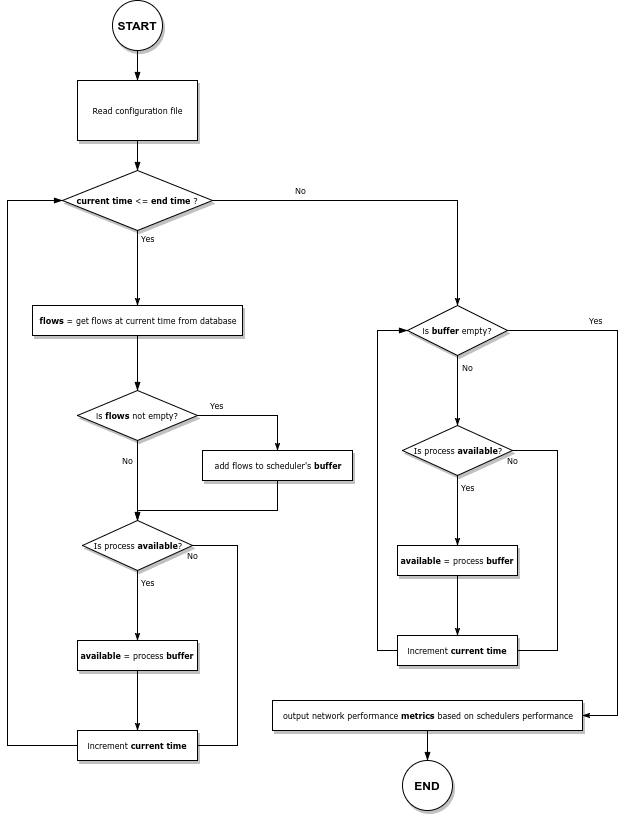
\includegraphics[width=\textwidth]{UNQS_FlowChart}
\label{fig:flowchart}\caption{\textbf{UNQS Main Program Logic}}
\end{figure*}

\section{Results and Discussion}

\subsection{Traffic Description}

Network traffic was collected from November 13-20. There were a total of 554,392 flows, 432,616,056 packets, and 2,297,393,747,224 bits observed in a period of 7.71 days (computed as the difference between the maximum \texttt{FIRST\_SWITCHED} minus the minimum \texttt{FIRST\_SWITCHED}, both written in Unix timestamp). The overall bandwidth of the observed traffic is tabulated below.

The top destination IP addresses for out-flow traffic are shown in Table \ref{top-out-flows} and the top source IP addresses for in-flow traffic are seen in Table \ref{top-in-flows}.

\begin{table*}[ht]
\centering
\caption{\textbf{Top 9 Out-Flows}}
\label{top-out-flows}
\begin{tabular}{|c|c|c|}
\hline
\textbf{DESTINATION (\# of flows)} 		& \textbf{TOTAL BYTES} 	& \textbf{\%} \\ \hline
	KDDI CORPORATION (1)				&  62409079786			& 60.6        \\ \hline
	MULTICAST (3)						&  12310903701          & 11.9        \\ \hline
	Google LLC(3)						&  5202456530           & 5.0         \\ \hline
	Facebook, Inc. (1)					&  2771346197           & 2.7         \\ \hline	
	Apple Inc.(1)						&  1054547100           & 1.0         \\ \hline
\end{tabular}
\end{table*}

\begin{table*}[ht]
\centering
\caption{\textbf{Top 9 In-Flows}}
\label{top-in-flows}
\begin{tabular}{|c|c|c|}
\hline
\textbf{SOURCE (\# of flows)} 		& \textbf{TOTAL BYTES} 	& \textbf{\%} \\ \hline
    KDDI CORPORATION(1)				&  79135454093			& 43.0        \\ \hline
    Google LLC(3)					&  27958817762          & 15.2        \\ \hline
    WorldStream B.V.(1)				&  3426880570           & 1.9         \\ \hline
    M247 Ltd(2)						&  4286472241           & 2.3         \\ \hline
    Converge ICT Solutions Inc.(2)	&  3967550023			& 2.2         \\ \hline    
\end{tabular}
\end{table*}

\begin{table*}[ht]
\centering
\caption{\textbf{Top 10 Destination Ports}}
\label{top-dest-ports}
\begin{tabular}{|c|c|c|c|}
\hline
\textbf{PORT NUMBER}			& \textbf{PROTOCOL}			& \textbf{TOTAL FLOWS}		& \textbf{\%} 	 \\ \hline
    443							& HTTPS						&  65088					& 11.7  	     \\ \hline
    53							& DNS						&  60765        			& 11.0			 \\ \hline
    1900						& SSDP						&  52579					& 9.5			 \\ \hline
    5060						& SIP						&  43101          			& 7.8   	     \\ \hline
    445							& Microsoft-DS				&  28746           			& 5.2        	 \\ \hline
    80							& HTTP						&  18485					& 3.3         	 \\ \hline
    5355						& LLMNR						&  17090    		        & 3.1    	     \\ \hline
    0							& Reserved					&  15732		            & 2.8       	 \\ \hline
    7437						& Faximum					&  13734        		    & 2.5         	 \\ \hline
    161							& SNMP						&  9142        			    & 1.6         	 \\ \hline
    67							& Bootstrap Protocol Server	&  8602        			    & 1.6         	 \\ \hline
\end{tabular}
\end{table*}

% IP addresses
Listed are brief descriptions for each company that is associated with the identified IP addresses.

\begin{enumerate}
\item \textbf{KDDI Corporation} is a telecommunications business based in Japan. It provides content hosting over optimized networks, and ICT and business services and solutions.

\item \textbf{Google LLC} is an American multinational technology company that specializes in Internet-related services and products such as online advertising technologies, search engine, cloud computing, software, and hardware.

\item \textbf{WorldStream B.V.} is a popular Internet Service Provider based in the Netherlands and is used by customers from all over the world. It provides cost-effective services to secure hosting environment, and offers hardware and Operating System technologies.

\item \textbf{M247 Ltd} is a UK-based technology company that offers  services and tools to secure network and data while providing connectivity and internet infastructure that expands to a global scale.

\item \textbf{Converge ICT} is a Philippine technology company with the fastest growing fiber internet and offers services to ensure pure end-to-end fiber internet connection, thus reducing data loss, faster speed and bandwidth.

\item \textbf{Facebook} is an American online social media and social networking service company.

\item \textbf{Apple Inc.} is an American multinational technology company that designs, develops, and sells consumer electronics, computer software, and online services. Multicast IPs allow group communication to be sent simultaneously to multiple computers.

\item \textbf{Multicast} * is not a company, but rather a form of data transmission that allows multiple hosts to receive data simultaneously.

\end{enumerate}

% references
%http://www.kddi.com/english/corporate/kddi/our-business/ may 28 2018
%https://www.worldstream.nl/en/about/company
%https://m247.com/about-us/
%http://www.convergeict.com/about-us/
%https://tools.ietf.org/html/rfc1112

% Ports

The Internet Assigned Numbers Authority (IANA) is responsible for associating port numbers with certain internet protocols used by network applications. These identifications can be found in IANA's \textit{Service Name and Transport Protocol Port Number Registry}. Table \ref{top-dest-ports} listed the top destination port numbers as recorded in the data. Each port number has a corresponding application protocol, which are as follows: 

% https://www.iana.org/assignments/service-names-port-numbers/service-names-port-numbers.txt

\begin{enumerate}

\item \textbf{Hypertext Transfer Protocol Secure (HTTPS)} - secures communication over a network

\item \textbf{Domain Name System (DNS)} - matches names to IP addresses and vice versa to facilitate network communications

\item \textbf{Simple Service Discovery Protocol (SSDP)} - advertises presence information to locate available network services

\item \textbf{Session Inititation Protocol (SIP)} - signals and controls multimedia communication sessions in Voice over IP (VoIP) applications like online voice and video calls

\item \textbf{Microsoft-Directory Services (MS-DS)} - follows the Server Message Block (SMB) protocol for shared access to files, printers, and serial ports and other communications between nodes on a network

\item \textbf{Hypertext Transfer Protocol (HTTP)} - facilitates data communication for the World Wide Web

\item \textbf{Link Local Multicast Name Resolution} - is based on DNS and allows both IPv4 and IPv6 hosts to perform name resolution for hosts on the same local links

\item \textbf{0 (Reserved)} and \textbf{7437 (Faximum)} - have no specifics protocols linked to them, and therefore are likely abused ports to send computer attacks and harmful computer and network content like viruses

\item \textbf{Simple Network Management Protocol (SNMP)} - collects and organizes information about managed devices on IP networks, and can modify information to change device behavior

\item \textbf{Bootstrap Protocol Server (BOOTP)} - exclusive protocol for IPv4; Dynamic Host Configuration Protocol (DHCP) server receives requests upon booting the client's computer

\end{enumerate}

%\linebreak
%\hrule

\subsection{Network Performance Metrics}

Three network performance metrics were accounted for as a result of the simulation, namely, duration, throughput, and flow loss. They are described in the items listed below.

\begin{enumerate}
\item \textbf{Duration}


Duration \textit{d} is a function of the arrival time \textit{t\textsubscript{0}} and last switched time \textit{t\textsubscript{n}} seen as follows:

\[
	d(t_0, t_n) = t_n - t_0
\]

\item \textbf{Throughput}

Throughput \textit{tput} was computed as 
\[
	tput = \frac{count(t_s)}{d}
\]

where \textit{t\textsubscript{s}} is the total size (in bytes) that was successfully switched, and \textit{d} as the computed duration. 

\item \textbf{Flow Loss}

The last network performance parametric looked at is the flow loss \textit{l}, solved by

\[
	l = \frac{count(f_d)}{count(f_d + f_s)} \times 100
\]

where all dropped flows \textit{f\textsubscript{l}} are counted and divided by the total number of flows \textit{f\textsubscript{d}} plus \textit{f\textsubscript{s}} (switched flows) multiplied by 100, to get the percentage. 

\end{enumerate}

\subsection{Simulation Results}

Simulation was run for the bandwidth settings 32.5 Mbps, 35.0 Mbps, 37.5 Mbps, 40 Mbps, and the timeout was set as a constant of 60 seconds.

Table \ref{simulation_res_per_bw} contains a summary of the simulation using the network performance metrics as defined in the previous section. It is observed that as the bandwidth is increased, the flows being dropped reduced while the flows being switched increased and became flat. Aside from the information concerning the flows, the simulation results showed that the througput and duration values across the four bandwidth constraints have significantly small difference and thus have similar performance.

\begin{table*}[ht]
\centering
\caption{\textbf{Simulation results per bandwidth}}
\label{simulation_res_per_bw}
\begin{tabular}{|c|c|c|c|c|}
\hline
                                  & \multicolumn{4}{c}{\textbf{BANDWIDTH (Mbps)}} \\ \hline
\textbf{METRICS}                  & \textbf{32.5}   & \textbf{35.0}  & \textbf{37.5} & \textbf{40.0}   \\ \hline
\textbf{flows\_dropped\_size (Gb)}  & 72.59           & 18.87 & 0& 0   \\ \hline
\textbf{flows\_dropped\_cnt}        & 36              & 9& 0& 0   \\ \hline    
\textbf{flows\_switched\_size (Gb)} & 866.46          & 920.18 &939.05 & 939.05    \\ \hline
\textbf{flows\_switched\_cnt}       & 554,356         &554,383&554,392&554,392
    \\ \hline
\textbf{duration (days)}          & 8.22            & 8.22& 8.22&8.22    \\ \hline
\textbf{throughput (Mbps)}        & 1.2             & 1.3& 1.3& 1.3    \\ \hline
\end{tabular}
\end{table*}


\section{Conclusion and Recommendation}

Traffic data that was collected using \texttt{ntopng} was successfully processed using the FIFO scheduling algorithm as simulated by UNQS. The output performance metrics showed the effect of increasing the bandwidth in order to switch all the flows. It was observed that the actual traffic data had a throughput of 3.45 Mbps. This value was used as a starting point to find out the probable advised bandwidth setting. After several attempts in varying the bandwidth constraint with intervals of 500 Kbps, the shift in the network performance metrics was observed between 35.0 Mbps and 37.5 Mbps.  While there were dropped flows under bandwidth constraint 35 Mbps, there was none under a bandwidth of 37.5 Mbps. The results for 32.5 Mbps and 40.0 Mbps were included to have an additional data for a better view of the emerging pattern. Therefore it is concluded that with the existing traffic data, a bandwidth of 37.5 Mbps is recommended as the most optimal.

Recommendations based on the analysis of the traffic data that was collected are listed below.
\begin{enumerate}
\item Block ports that are still not tagged by the firewall, like ports 0 and 7437, which have potential receive harmful traffic data.
\item Maintain and use an internal DNS server to further reduce external DNS traffic.
\item Turn off MS-DS traffic that consumes a large amount of the out-bound bandwidth.
\item Mirror Linux, Microsoft, and Apple traffic to monitor possible intrusions and unnecessary traffic within the network in order formulate and enforce policies to block and limit such traffic.
\end{enumerate}

Future works may explore more complex scheduling algorithms aside from the native FIFO queueing algorithm like PQ and WFQ in order to determine more optimal scheduling techniques that will minimize the bandwidth constraint and save expenses. Additionally, data could be collected over a longer time period to discover a pattern in network traffic behavior depending on certain periods of time, such as peak season during enrollment period, etc.. Doing so could give a better picture of the maximum bandwidth usage and thus determine the optimal, cost-efficient, and effective bandwidth setting, which can be paired with a queueing technique for further cost reductions and improved performance.

% BIBLIOGRAPHY
\bibliographystyle{./IEEE/IEEEtran}
\bibliography{./cs190-ieee}
% \nocite{*}

% BIOGRAPHY
\begin{biography}[{
\includegraphics{./yourPicture.eps}}]{\ADVISEE}
She is a BS Computer Science undergraduate student. She not only writes code, but also songs, poems, and stories.
\end{biography}

\end{document}
